\subsection{Heading Angle}
The heading angle is one of the parameters of interest for the project, partly because it is relevant in the development of the driver model, and partly because it helps enhance the other calculations that will follow (i.e. lateral offset and longitudinal range). Three methods for calculating the heading angle are introduced here, although only the first method is used for the development of the tool.

\subsubsection{Method 1 for Heading Angle: Triangulation}
After identifying the vanishing point and rectifying the image for intrinsic and extrinsic parameters, one can transform points on the picture from the 2D view to a 3D view, as long as one of the coordinates is known. For the sake of this project, the transformations will be on the ground plane, meaning that the Z-component of the points to be calculated is known and equal to the height of the camera above the ground. The following figure depicts what is meant by transforming the view from 2D to 3D coordinates.

\begin{figure}[H]
    \centering
    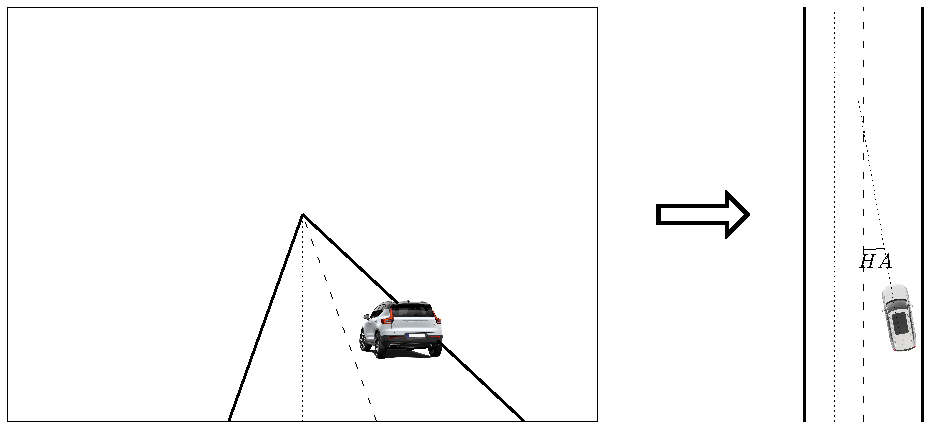
\includegraphics[width=\textwidth]{Figures/2d2d3.pdf}
    \caption{2D to 3D transformation}
    \label{fig:2d23d}
\end{figure}


In order to change from 2D to 3D coordinates, the following method can be used starting with calculating the Y-coordinate (longitudinal distance) of a ground point and then its X-coordinate) lateral offset.

\begin{figure}[H]
    \centering
    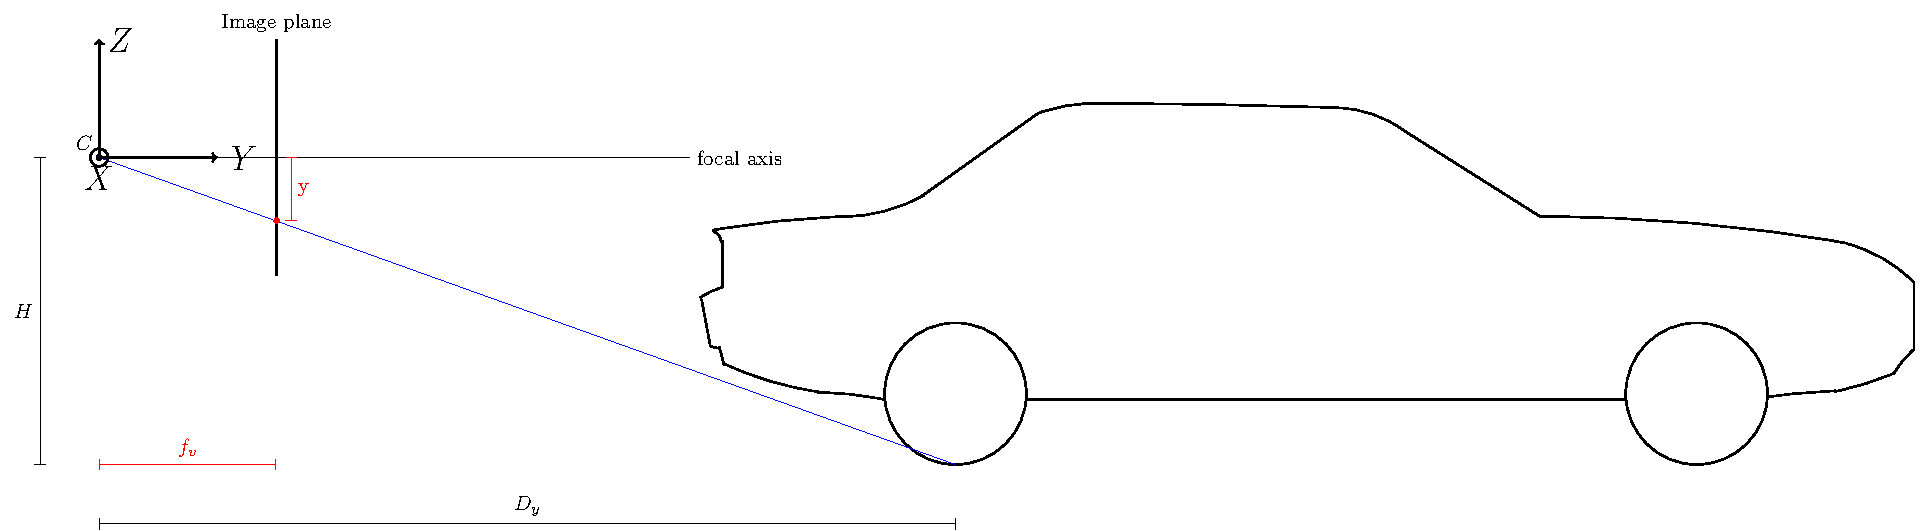
\includegraphics[width=\textwidth]{Figures/D_y.pdf}
    \caption{Distance calculation in $yz$-plane of vehicle reference frame}
    % \label{fig:my_label}
\end{figure}

\begin{equation}
    \frac{D_y}{H} = \frac{f_v}{y} \Rightarrow D_y = \frac{H f_v}{y}
\end{equation}



\begin{figure}[H]
    \centering
    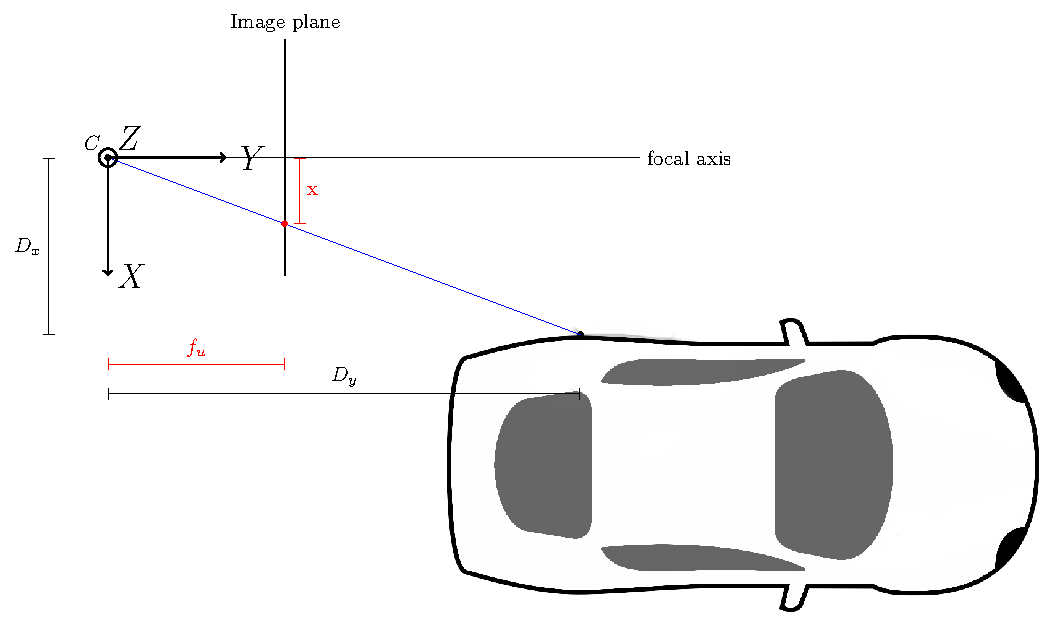
\includegraphics[width=\textwidth]{Figures/D_x.pdf}
    \caption{Distance calculation in $xy$-plane of vehicle reference frame}
    % \label{fig:my_label}
\end{figure}

\begin{equation}
    \frac{D_y}{D_x} = \frac{f_u}{x} \Rightarrow D_x = \frac{D_y x}{f_u} = \frac{H f_v x}{f_u y}
\end{equation}

The coordinates in 3D of the wheels can now be expressed as
\begin{equation*}
    \begin{bmatrix}
    X\\Y\\Z
    \end{bmatrix}
    =
    \begin{bmatrix}
    D_x\\D_y\\-H_{camera}
    \end{bmatrix}
\end{equation*}

Using the X and Y coordinates of the two wheels, one can get the equation of the line joining the two wheels and by getting the slope of this line one can easily calculate the heading angle of the POV. The heading angle is hence

\begin{equation}
    HA = \psi_{POV} = -tan^{-1} \left( \frac{X_1 - X_2}{Y_1 - Y_2} \right)
\end{equation}

\subsubsection{Method 2 for Heading Angle: Number plate}
This method is suggested by the team members but not used in the project. It was also not found to be used in other research either. The method can be described as follows: using the number plate of a car, which has a standard shape and size, one can check the edges of the plate and calculate the size and angles shown in the picture. Based on that, one can get the heading angle of the vehicle. This method may not be the best way to follow, due to the limited quality of the videos available in the dataset.

\subsubsection{Method 3 for Heading Angle: Side plane homography}
This method is also based on the homography concept. By checking the change in the homography of the side of the car and tracking this plane as the car moves, one can achieve the rotation of this plane relative to the camera and hence the relative heading angle of the POV. This method has several difficulties, especially the translation of the camera, and is to be investigated in future work.

\subsection{Lateral Offset}
The lateral offset is another important parameter for developing a driver model. In fact, the lateral distance to the lane marking and the "speed of attack" of the POV towards the lane line are of paramount interest in this project. Two methods for estimating the lateral offset of the POV are discussed here.

\subsubsection{Method 1 for Lateral Offset: Pixel width}
Using the pixel size of the rear end of the vehicle, one can get the distance from the center of the vehicle to the focal axis of the camera. This is solved by a system of 2 equations where the unknown variables are the lateral offset $L$ and the range of the car $D$.

\begin{figure}[H]
    \centering
    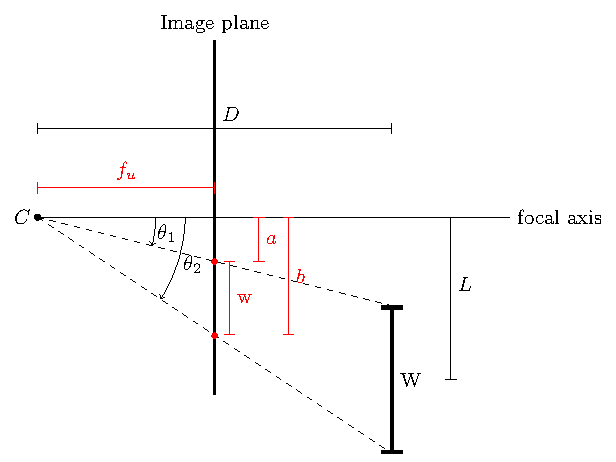
\includegraphics[width = 0.8\textwidth]{Figures/DistanceCalc.pdf}
    \caption{Distance calculation using pixel width method}
    % \label{fig:my_label}
\end{figure}

\begin{equation}
    \frac{a}{f_u} = tan\left( \theta_1 \right) =  \frac{L - \frac{W}{2}}{D} \label{eq:dista}
\end{equation}
\begin{equation}
    \frac{b}{f_u} = tan\left( \theta_2 \right) = \frac{L + \frac{W}{2}}{D} \label{eq:distb}
\end{equation}

By solving the system of equations above, we get the following results:
\begin{equation}
    D = \frac{W f_u}{b-a} \label{eqn:distD}
\end{equation}
\begin{equation}
    L = \frac{W}{2} \left( \frac{a+b}{b-a}\right) \label{eqn:distL}
\end{equation}

In some cases, the POV will have a certain heading angle, which will cause the pixel width $w = b-a$ to seem smaller than what it is in reality. To account for that, the heading angle should be incorporated in the pixel width $w$ such that
\begin{equation}
    w' = \frac{w}{cos(\psi_{POV})} \label{eqn:w_withheading}
\end{equation}

It is important to note that this method gives the relative distances of the POV with respect to the camera's center. In order to get the lateral offset of the POV to the lane, further development of this method is required where the position of the SV in its lane in known.

\subsubsection{Method 2 for Lateral Offset: Triangulation}
Using a similar approach to what was explained earlier, one can get the 3D coordinates of the contact between the wheels and the ground ($X_w,Y_w,Z_w$). Also, getting the equation of the lane line in 3D follows the same method. With the wheel coordinates and the lane line equation in hand, it becomes simple to get the distance between the wheels and the lane. This approach is in fact a simple 2D calculation since all the points lie on the ground plane. The equation used to get the distance between the points and the lane line is:
\begin{equation}
    lateralDistance = \frac{m X_w - Y_w + b}{\sqrt{a^2+1}}
\end{equation}
where the equation of the lane line in the ground plane is $Y = mX+b$.

By deriving the resultant distance with respect to time (i.e. dividing the change in the lateral distance by the time step of each frame), the lateral offset speed and the "speed of attack" of the POV towards the lane line are obtained.

\subsubsection{Error Estimation}
The two methods mentioned above rely on assumptions that affect the accuracy and precision of the results. To check the performance of the tool, the resultant distances will be compared to radar data that is available for the dataset in hand. The errors are hence calculated based on the difference between the output of the tool and the radar data.

Those errors are caused by the following assumptions:
\begin{itemize}
    \item Width of POV
    \item Length of trunk of POV
    \item Camera's height
    \item SV's hood length
    \item Extrinsic parameters (pitch and yaw angles of camera)
    \item Manual selection of the POV's rear and wheels as well as the manual selection of points on the lane lines
    \item Interpolation between frames
\end{itemize}

